\chapter{Introduction}
\label{chap:intro}
\lhead{\emph{Introduction}}

Imagine never having to search through disorganized notes or wonder if you saved that crucial PDF from last week’s lecture. NoteReader will address the core challenges of disjointed learning resources and disconnected note-taking, offering a unified platform that promotes better learning, better organization, and better revision.

NoteReader is a study solution that provides an all-in-one interface for document reading and note-taking. By supporting a wide range of file types, including PDFs, Word documents, PowerPoint slides, and eBooks, allowing users to seamlessly organize their study material and notes side-by-side. 

The core interface of NoteReader is the Split-View. Each time the user opens a document a dedicated folder is created in the user's file system to store notes linked directly to the document and its page number. The document is displayed on the left pane of the window, while a text editor is displayed on the right. On returning to NoteReader, previously viewed documents will be accessible via a catalogue/ library. 

The note editor will support Markdown and HTML, allowing users to create rich, formatted notes. As users navigate through the document, new notes are created automatically for each page. If a user returns to a previous page, the corresponding note is instantly loaded in the editor. Optionally pages can be merged to allow for a more seamless experience. 

Notes are stored in lightweight plain-text files, they are inherently portable ensuring compatibility with other tools like Obsidian. Notes are saved in real time and can be automatically synced to version control providers like GitHub, giving users access to version-controlled notes across devices. 

Features such as document cataloguing, page-specific notes, and a robust tagging system make it easy for users to locate specific information. Advanced features like handwriting support and time-stamped notes for videos and audiobooks are planned as potential stretch goals.


\section{Motivation}

You are revising for an exam. You open a lecture slide on your laptop, but where are your notes? Are they on Google Docs, in OneNote, or saved as scattered files on your desktop? For many students, this process is repetitive and inefficient. Modern note-taking tools do not treat source material as a first-class priority. Instead, they focus on creating isolated notes with minimal connection to the material being studied.

\begin{figure}
    \centering
    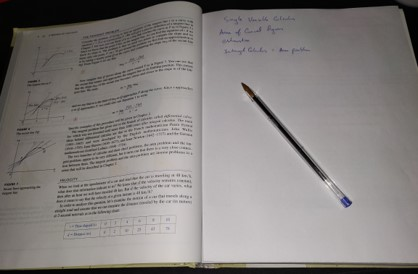
\includegraphics[width=0.5\linewidth]{Figures/book.jpg}
    \caption{A book with a blank sheet of paper slotted between the pages to take notes on}
    \label{fig:enter-label}
\end{figure}

Picture a book with a blank sheet of paper slotted in between each page. As you read, you take notes on this paper and as you flip to the next page, a new sheet awaits you. When it’s time to revise, you go back to that page of the book and the sheet containing your notes on the topic are right there waiting for you.  

No flipping between refill pads, copy-books, documents on your laptop, or in the cloud. No wondering if the notes you took are complete, or if you missed an important point. Everything is in one place. 

Now combine this with digital document management and cataloguing, tagging, searching and linking. It should be trivial to find your notes when you need to refer back. 

This is the feeling note reader wants to achieve. 

Note reader aims to reduce the friction associated with storing and accessing notes and study material. Reduce the cognitive load of note-taking and encourage real-time engagement with the material. 

\section{Contribution}

The application proposed in this project is composed of several key features, such as document reading and rendering, text editing, cataloguing and multiplatform support. To orchestrate these components in a seamless manner, I will leverage the skills and knowledge gained throughout my degree program. 

I will apply user-centred design principles through requirements engineering to ensure NoteReader addresses the clear needs of its intended users. This includes gathering, prioritizing, and validating functional and non-functional requirements.

Adherence to object-oriented design principles (like encapsulation, abstraction, inheritance, and polymorphism) will ensure a cohesive, modular system. Core functionalities like document viewing, note synchronization, and user interaction will be implemented as modular, reusable components.

By following object-oriented design principles, NoteReader will be maintainable and extensible. Changes to one part of the system (like file type support) can be isolated to specific classes or components without affecting the rest of the application. This modular approach ensures scalability as new features are introduced.

NoteReader will be developed using the agile Scrum framework, focusing on iterative development. Emphasis will be placed on early delivery of a minimum viable product (MVP) with successive prototype releases. These iterations will allow for continuous feedback loops and improvement.

Knowledge of agile methodologies will enable me to manage project scope, prioritize features, and ensure timely delivery of new prototypes. Skills in backlog management, sprint planning, and stakeholder collaboration will be demonstrated through well-documented sprints and the inclusion of a feedback process for user testing.

Since NoteReader is a multiplatform solution, user accessibility across devices is a core requirement. The UI must adapt to multiple screen sizes and input methods (desktop, tablet, mobile). By using Kotlin Multiplatform, I will leverage platform-specific adaptations for mobile and desktop environments.

The application will maintain a consistent user experience (UX) across Windows, macOS, Linux, and mobile devices. Designing UI components that work equally well on different devices will showcase the skills I gained from mobile development modules. The ability to seamlessly handle document navigation and note creation across platforms is central to NoteReader's usability.

One of NoteReader's unique value propositions is the use of version control services (like GitHub and GitLab) as a method of synchronizing notes. This method ensures that users have access to their notes across multiple devices while maintaining a revision history of their notes.

This feature demonstrates my ability to develop tools that leverage existing cloud infrastructure to deliver a seamless synchronization experience. My knowledge of Git API integration will allow me to build features for automatic sync, conflict resolution, and file version tracking.

A No-SQL file-system-based approach will be used to store and organize notes, metadata, and links to source documents. This approach provides flexibility in handling diverse data formats (PDFs, Word documents, PowerPoints, etc.) and ensures that all associated notes are easily searchable.

The catalogue file (or index) will be synced alongside the notes themselves in the Git repository. This ensures that the state of the catalogue remains synchronized with user notes, even when accessed from multiple devices.

By using Git for note synchronization, the catalogue must be resilient to merge conflicts and data corruption. The system will be designed to track changes to catalogue files, and where conflicts arise, the system will attempt to resolve them automatically or rebuilding, alerting the user only if manual intervention is required.

\section{Structure of This Document}

This document is organized into the following sections:

\begin{table}[h!]
\centering
\begin{tabular}{|p{5cm}|p{10cm}|}
\hline
\textbf{Section} & \textbf{Description} \\ \hline
Introduction & Outlines the motivation behind the project, the key contributions, and an overview of the document's structure. \\ \hline
Background & Provides context for the project, including its thematic position within computer science, a review of existing solutions, and relevant literature on the topic of digital note-taking and learning efficiency. \\ \hline
Problem Definition & Discusses the core challenges that the project seeks to address, outlining existing issues with current solutions and presenting the objectives and functional requirements of the proposed application. \\ \hline
Implementation Approach & Details the methodology used to develop the application, including user flows, architectural design, technologies, risk assessment, and the implementation timeline. \\ \hline
Implementation & Details the actual implementation of the project and difficulties encountered. \\ \hline
Testing and Evaluation & Breaks down the methods used to evaluate progress \\ \hline
Conclusions and Future Work & Summarizes the findings and learnings of the project, reflects on the challenges encountered, and outlines potential future developments. \\ \hline
Appendices & Includes supplementary materials such as code snippets, wireframe models, and diagrams to support the main text. \\ \hline
\end{tabular}
\caption{Structure of This Document}
\label{tab:document_structure}
\end{table}


